% Drawing 141/01-3 -- folder 141, batch 01, archive page 9 (PDF page 10).
% Transcription: l'ellipse décrite dans le texte : deux croix à gauche, marquées $0$ et \uncertain{$2^{3}\cdot 3^{4}$}, un gros point à droite, deux marques épaisses en pointe de flèche sur le bord (en bas et en haut à droite) ; au-dessus un court trait horizontal, à gauche un trait vertical interrompu, à droite « $C_{1,1}$ ».
% Kind: ellipse with two crosses, a point and arrow marks on its rim. Method 2 (schematic redraw from the facsimile). Status: partial.
% Notes: The ellipse; inside, two small crosses at the left with their labels below them, 0 and the product read 2^3.3^4 by the transcription (uncertain there; kept), and a heavy point at the right; on the rim a heavy arrow mark at the bottom (pointing right) and a heavy tick at the upper right; above the ellipse a short horizontal stroke with a heavy end on each side; at the left a broken vertical stroke; at the right the label C_{1,1}. Still differs: the two rim marks are drawn as short heavy strokes with a head on the lower one; whether the upper one is an arrowhead is not clear. The transcription describes this figure in an editorial sentence of the text (« Une ellipse marquée de deux croix ... ») and had no mark for it. Redrawn 2026-11-12 (issue 128): to check again.
% Coordinates: 1 unit = 0.6 mm = 1/100 of the crop width (bbox in page fractions: [0.22, 0.49, 0.45, 0.59]).
% Redrawn by Claude (claude-fable-5-2), issue #128, 2026-11-12; not checked by a human; not compiled (no TeX in the session).
% Rights: reproduces part of the work -- behind RENDER_TRANSCRIPTS, never published by itself.
\documentclass[tikz,border=3pt]{standalone}
\usepackage{amsmath,amssymb}
\usetikzlibrary{patterns,arrows.meta}
\tikzset{pencil/.style={black!45}, struck/.style={black!35}, mpt/.style={circle,draw,inner sep=1.3pt}, pt/.style={circle,fill,inner sep=0.9pt}, opt/.style={circle,draw,fill=white,inner sep=1.1pt}}
\begin{document}
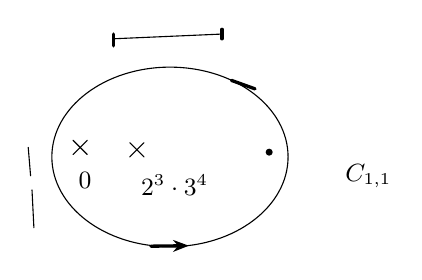
\begin{tikzpicture}[x=0.6mm,y=0.6mm,line cap=round,line join=round,font=\scriptsize]
\draw (37,-37) ellipse[x radius=25, y radius=19];
\draw (16.5,-33.5) -- (19.5,-36.5);
\draw (19.5,-33.5) -- (16.5,-36.5);
\draw (28.5,-34) -- (31.5,-37);
\draw (31.5,-34) -- (28.5,-37);
\node[inner sep=1pt] at (19,-42) {\small $0$};
\node[inner sep=1pt] at (38,-43) {\small $2^{3}\cdot 3^{4}$};
\node[pt] at (58,-36) {};
\draw[very thick,-{Stealth[length=2mm]}] (33,-55.9) -- (41,-55.8);
\draw[very thick] (50,-20.8) -- (55,-22.6);
\draw (25,-12) -- (48,-11);
\draw[very thick] (25,-11) -- (25,-13.5);
\draw[very thick] (48,-10) -- (48,-12);
\draw (7,-35) -- (7.5,-41);
\draw (7.8,-44) -- (8.2,-52);
\node[inner sep=1pt] at (79,-41) {\small $C_{1,1}$};
\end{tikzpicture}
\end{document}
